\documentclass{standalone}
\usepackage{tikz}
\usepackage{pgfplots}
\pgfplotsset{compat=1.18}
\usepgfplotslibrary{groupplots}
\usetikzlibrary{fadings,shadings,calc}

% Shape rendering specs
\pgfdeclareradialshading{atomshade}{\pgfpoint{0cm}{0cm}}{%
    color(0cm)=(pgftransparent!0);
    color(0.2cm)=(pgftransparent!20);
    color(0.5cm)=(pgftransparent!50);
    color(0.7cm)=(pgftransparent!70);
    color(1cm)=(pgftransparent!100)%
}

\tikzset{
    atom/.style={circle, shading=atomshade, minimum size=0.4cm},
    bond/.style={
        line width=0.5mm,
        shading=axis,
        color=black, %Change to #1 to specify bond color
        shading angle=45
    }
}

% Define BaTiO3 (#221) unit cell projection
\newcommand{\DrawUnitCell}[1]{%
    \begin{tikzpicture}[scale=1.5]
    % Draw the unit cell
    \draw[thick] (0,0,0) -- (1,0,0) -- (1,1,0) -- (0,1,0) -- cycle; % Bottom face
    \draw[thick] (0,0,1) -- (1,0,1) -- (1,1,1) -- (0,1,1) -- cycle; % Top face
    \draw[thick] (0,0,0) -- (0,0,1);
    \draw[thick] (1,0,0) -- (1,0,1);
    \draw[thick] (1,1,0) -- (1,1,1);
    \draw[thick] (0,1,0) -- (0,1,1);

    % Draw lines connect Oxygen to Titanium
    \begin{scope}
        \ifnum \pdfstrcmp{#1}{0.5} < 0
            % Connect bottom 4 oxygens to Ti
            \draw[bond=red] (0,0.5,0.5) -- ($(0,0.5,0.5)!0.5!(0.5,#1,0.5)$);
            \draw[bond=gray] ($(0,0.5,0.5)!0.5!(0.5,#1,0.5)$) -- (0.5,#1,0.5);
            \draw[bond=red] (1,0.5,0.5) -- ($(1,0.5,0.5)!0.5!(0.5,#1,0.5)$);
            \draw[bond=gray] ($(1,0.5,0.5)!0.5!(0.5,#1,0.5)$) -- (0.5,#1,0.5);
            \draw[bond=red] (0.5,0,0.5) -- ($(0.5,0,0.5)!0.5!(0.5,#1,0.5)$);
            \draw[bond=gray] ($(0.5,0,0.5)!0.5!(0.5,#1,0.5)$) -- (0.5,#1,0.5);
            \draw[bond=red] (0.5,0.5,0) -- ($(0.5,0.5,0)!0.5!(0.5,#1,0.5)$);
            \draw[bond=gray] ($(0.5,0.5,0)!0.5!(0.5,#1,0.5)$) -- (0.5,#1,0.5);
            \draw[bond=red] (0.5,0.5,1) -- ($(0.5,0.5,1)!0.5!(0.5,#1,0.5)$);
            \draw[bond=gray] ($(0.5,0.5,1)!0.5!(0.5,#1,0.5)$) -- (0.5,#1,0.5);
        \else
            \ifnum \pdfstrcmp{#1}{0.5} > 0
                % Connect top 4 oxygens to Ti
                \draw[bond=red] (0,0.5,0.5) -- ($(0,0.5,0.5)!0.5!(0.5,#1,0.5)$);
                \draw[bond=gray] ($(0,0.5,0.5)!0.5!(0.5,#1,0.5)$) -- (0.5,#1,0.5);
                \draw[bond=red] (1,0.5,0.5) -- ($(1,0.5,0.5)!0.5!(0.5,#1,0.5)$);
                \draw[bond=gray] ($(1,0.5,0.5)!0.5!(0.5,#1,0.5)$) -- (0.5,#1,0.5);
                \draw[bond=red] (0.5,1,0.5) -- ($(0.5,1,0.5)!0.5!(0.5,#1,0.5)$);
                \draw[bond=gray] ($(0.5,1,0.5)!0.5!(0.5,#1,0.5)$) -- (0.5,#1,0.5);
                \draw[bond=red] (0.5,0.5,1) -- ($(0.5,0.5,1)!0.5!(0.5,#1,0.5)$);
                \draw[bond=gray] ($(0.5,0.5,1)!0.5!(0.5,#1,0.5)$) -- (0.5,#1,0.5);
            \else
                % Connect 8 oxygens to form octahedron
                \draw[bond=red] (0,0.5,0.5) -- (1,0.5,0.5);
                \draw[bond=red] (0.5,0,0.5) -- (0.5,1,0.5);
                \draw[bond=red] (0.5,0.5,0) -- (0.5,0.5,1);
            \fi
        \fi
    \end{scope}

    % Draw the Oxygen atoms (Red) (back perspective)
    \node[atom, anchor=center,ball color=red] at (0,0.5,0.5) {};
    \node[atom, anchor=center,ball color=red] at (0.5,0,0.5) {};
    \node[atom, anchor=center,ball color=red] at (0.5,0.5,0.0) {};

    % Draw the Barium atoms (Cyan)
    \node[atom, anchor=center,ball color=cyan] at (0,0,0) {};
    \node[atom, anchor=center,ball color=cyan] at (1,0,0) {};
    \node[atom, anchor=center,ball color=cyan] at (0,1,0) {};
    \node[atom, anchor=center,ball color=cyan] at (1,1,0) {};
    \node[atom, anchor=center,ball color=cyan] at (0,0,1) {};
    \node[atom, anchor=center,ball color=cyan] at (1,0,1) {};
    \node[atom, anchor=center,ball color=cyan] at (0,1,1) {};
    \node[atom, anchor=center,ball color=cyan] at (1,1,1) {};

    % Titanium atom (Gray)
    \node[atom, anchor=center,ball color=gray, minimum size=0.25cm] at (0.5,#1,0.5) {};

    % Draw the Oxygen atoms (red) (front perspective)
    \node[atom, anchor=center,ball color=red] at (0.5,1,0.5) {};
    \node[atom, anchor=center,ball color=red] at (1,0.5,0.5) {};
    \node[atom, anchor=center,ball color=red] at (0.5,0.5,1) {};

    \end{tikzpicture}%
}

\begin{document}
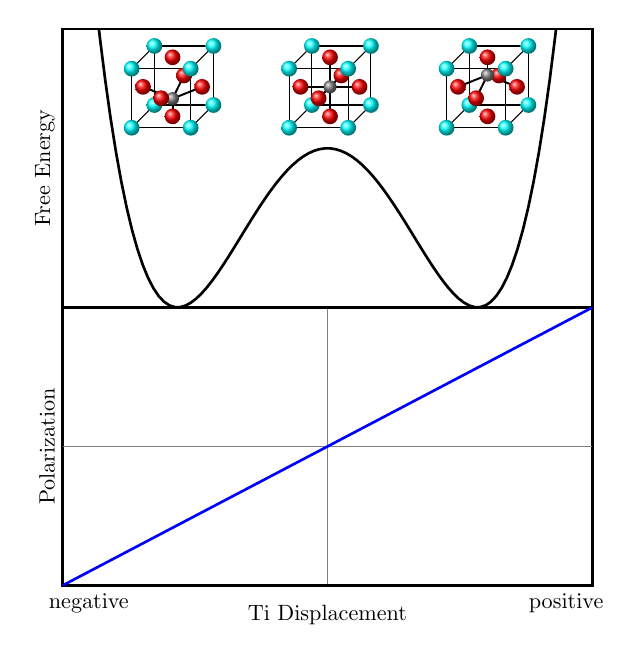
\begin{tikzpicture}[scale=0.8]
    % Define top and bottom plots
    \begin{groupplot}[
        group style={group size=1 by 2, vertical sep=0pt},
        width=10cm,
        height=6cm,
        xtick=\empty,
        ytick=\empty,
        axis lines*=box,
        enlargelimits=false,
        xmin=-2.5, xmax=2.5,
        axis line style={very thick},
    ]
        % Double-well free energy potential
        \nextgroupplot[
            ylabel={Free Energy},
            ylabel style={rotate=0},
            ymin=0, ymax=3.5,
            xlabel={}, % Remove x-axis label from top plot
            tick style={draw=none},
        ]
        \addplot[domain=-2.5:2.5, samples=100, very thick] {0.5*(\x^4-4*\x^2+4)};

        % Polarization vs. displacement
        \nextgroupplot[
            ylabel={Polarization},
            ylabel style={rotate=-90},
            ymin=-2.5, ymax=2.5,
            xlabel={Ti Displacement},
            xlabel shift={-10pt},
            xlabel near ticks,
            ylabel near ticks,
            xtick={-2.25, 2.25},
            xticklabels={negative, positive},
            tick style={draw=none},
        ]
        % Additional axes through origin
        \draw[black!50, thick] (axis cs:0,-2.475) -- (axis cs:0,2.475);
        \draw[black!50, thick] (axis cs:-2.49,0) -- (axis cs:2.49,0);

        % Polarization line
        \addplot[domain=-2.5:2.5, samples=2, blue, very thick] {\x};
    \end{groupplot}

    % Overlay the unit cells manually
    \node[anchor=center] at (1.75,3.5) {\scalebox{0.5}{\DrawUnitCell{0.3}}};
    \node[anchor=center] at (4.25,3.5) {\scalebox{0.5}{\DrawUnitCell{0.5}}};
    \node[anchor=center] at (6.75,3.5) {\scalebox{0.5}{\DrawUnitCell{0.7}}};
\end{tikzpicture}
\end{document}
